\section{Clickstream data: Interface participants' time spent}
In addition to distance, we analyzed time participants spent per option. We aggregated the total time participants spent per option using the QS system log. For participants in the two-phase interface conditions, this included both organization and voting times for that option. The results are visualized in Figure~\ref{fig:total_time}.

\begin{figure}[h]
    \centering
    % First subfigure
    \begin{subfigure}[b]{0.52\textwidth}
        \centering
        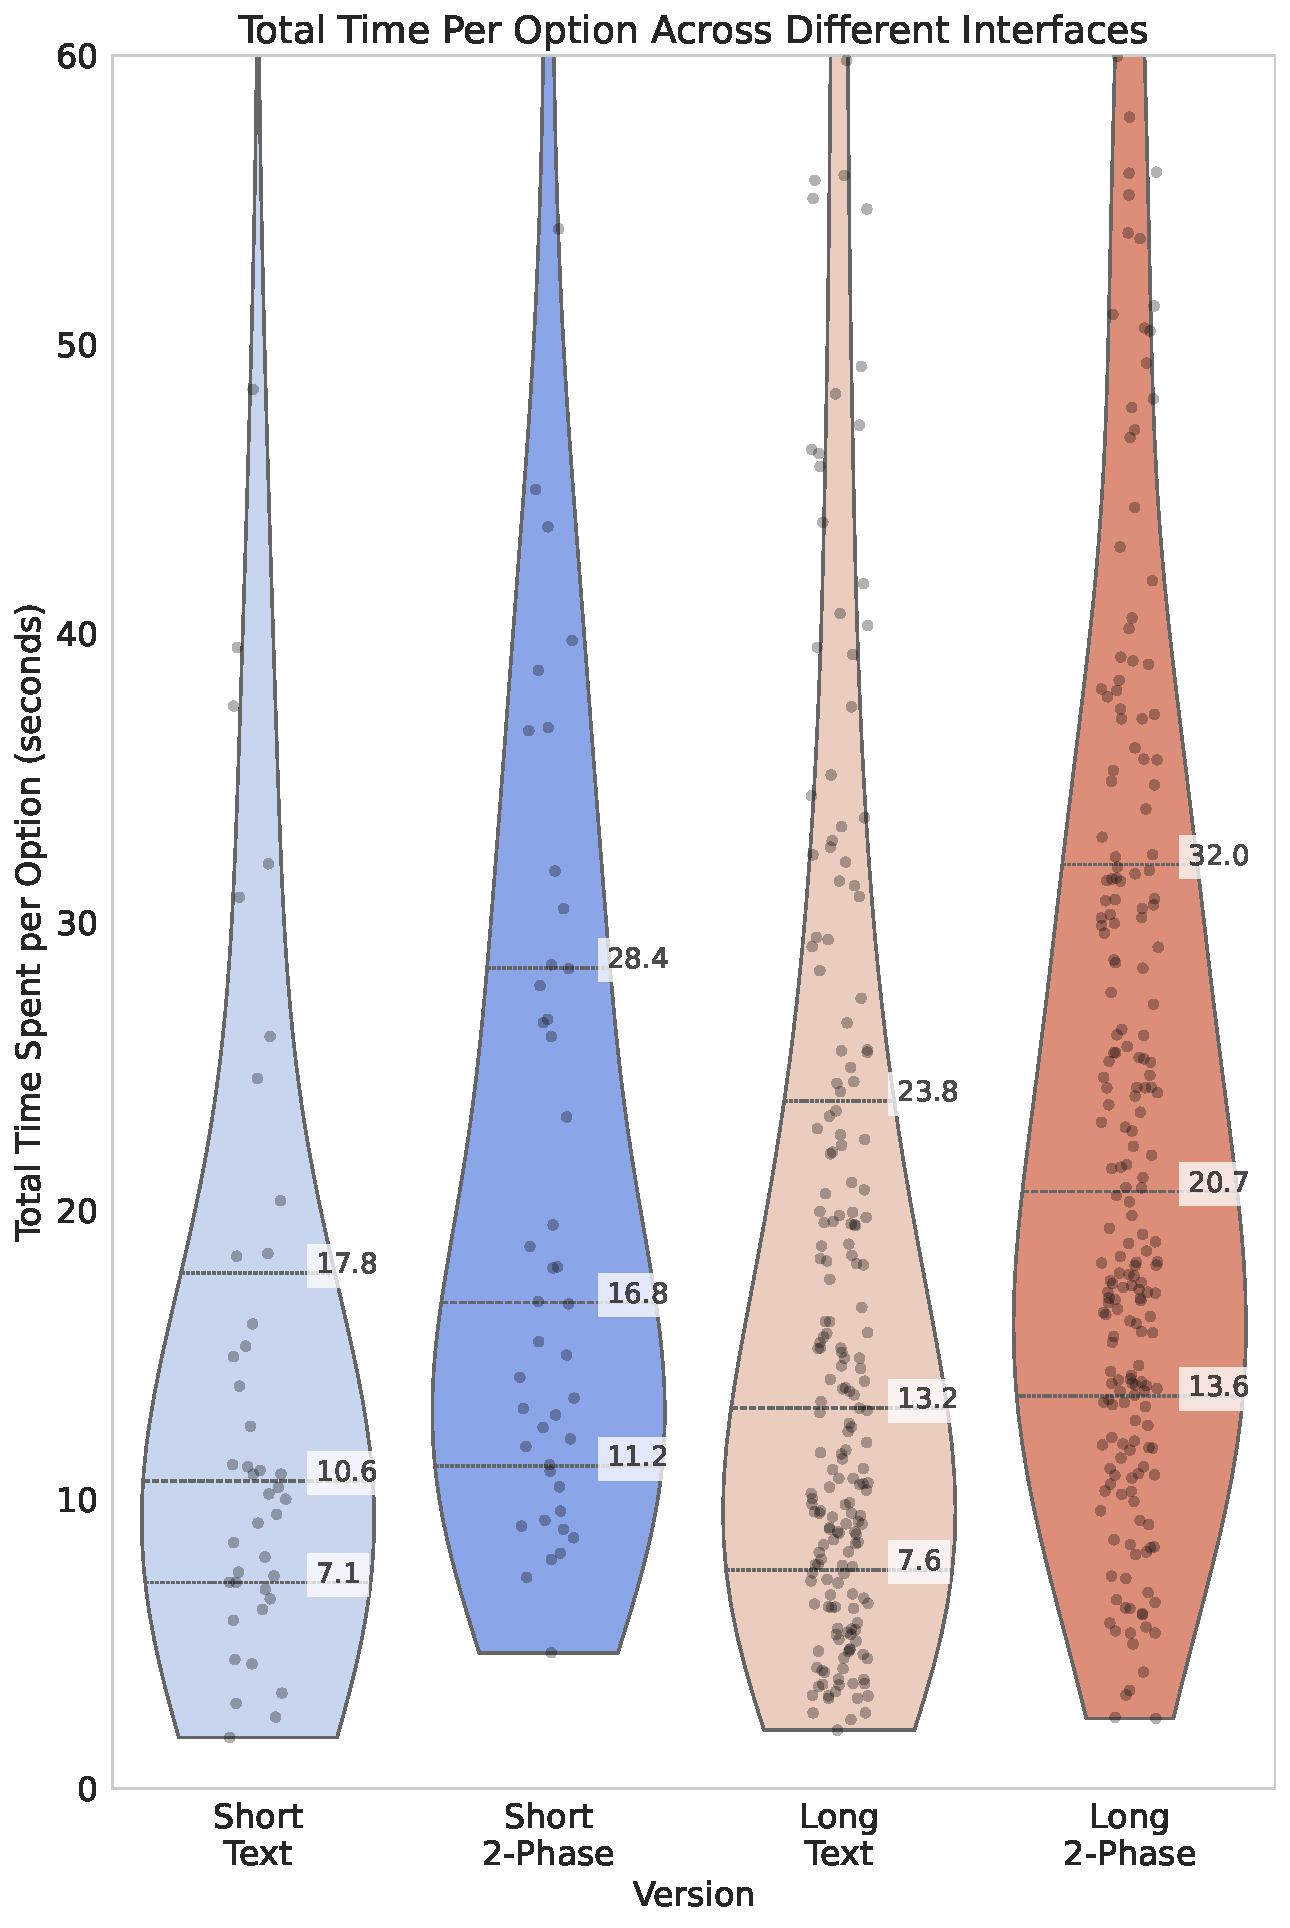
\includegraphics[width=0.95\textwidth, trim=0 10 0 10, clip]{content/image/results/total_time_per_option.pdf}
        \captionsetup{width=\textwidth, justification=justified} % Adjust the width to match the image width
        \caption{Total Time per option: We identified that the two-phase interface skewed slightly higher than the text interface, as expected. This discrepancy can be attributed to the extra organization step required in the two-phase interface, leading to a slightly longer overall completion time per option.}
        \Description{Violin plot showing total time spent per option in seconds across four interface versions: Short Text, Short 2-Phase, Long Text, and Long 2-Phase. The y-axis ranges from 0 to 60 seconds. Each violin plot has scattered dots representing individual data points. The shape of the Short Text plot is widest between 10 and 20 seconds, tapering at the top and bottom. The Short 2-Phase plot is the narrowest, with most dots concentrated between 10 and 20 seconds. The Long Text plot is narrow and widest near the bottom, between 5 and 15 seconds. The Long 2-Phase plot is widest near the top, between 20 and 40 seconds.}
        \label{fig:total_time}
    \end{subfigure}
    \hfill
    % Second subfigure
    \begin{subfigure}[b]{0.38\textwidth}
        \centering
        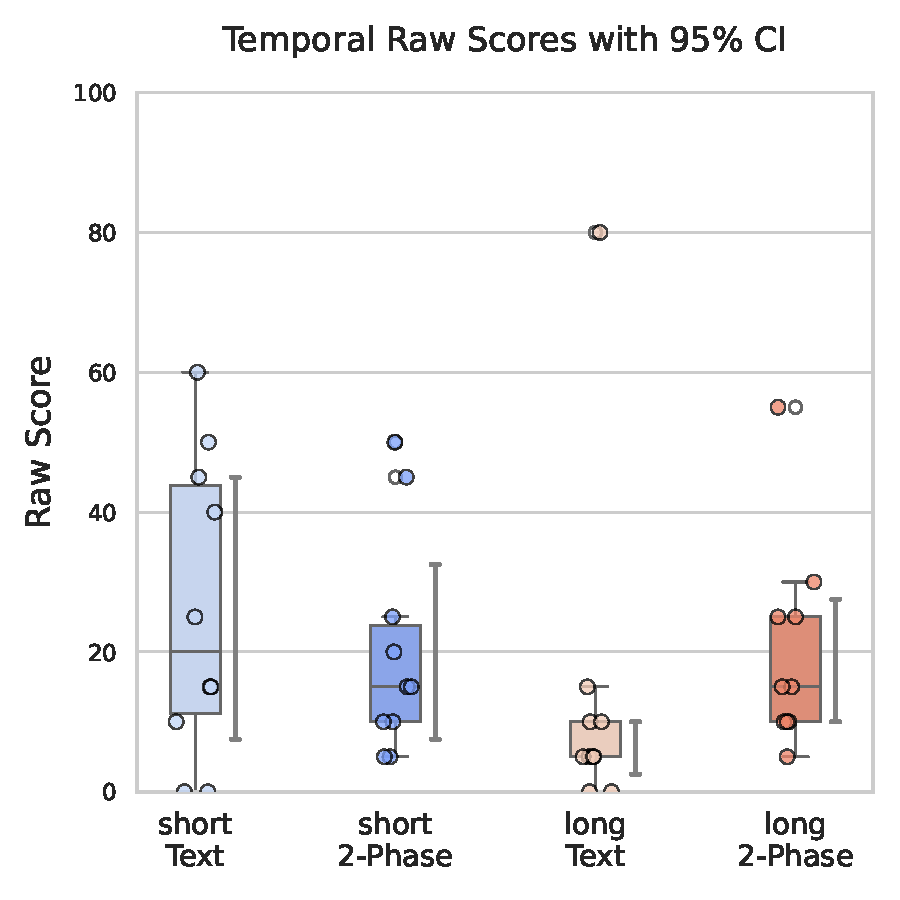
\includegraphics[width=0.95\textwidth, trim=0 13 0 13, clip]{content/image/cog/Temporal_scores.pdf}
        \captionsetup{width=\textwidth, justification=justified} % Adjust the width to match the image width
        \caption{Temporal Demand Raw Score: The short text interface results in the highest temporal demand, while the long text interface is the lowest. Two-phase interfaces show moderate temporal demand, suggesting that interactive elements allowed participants to pace themselves better.}
        \label{fig:temporal_cog_score}
    \end{subfigure}
\end{figure}

Overall, participants spent slightly more time per option in the two-phase interface than in the text interface. To quantify these observations, we modeled the time data using independent beta distributions within a Bayesian framework, assuming independence across experimental conditions. For example, participants using the long two-phase interface spent significantly more time per option than those using the long text interface (medium to large effect size, XX, d=XX), with an even more pronounced difference between the short two-phase and short text interfaces (medium effect size, XX, d=XX). These findings suggest that the interactive two-phase interface encourages longer deliberation, particularly for longer lists of options. Participants in both interfaces tended to spend more time per option with high probability. Details of the modeling procedure and priors are provided in Appendix XX.

Some literature points to increased time leading to time fatigue~\cite{}, which can impair decision making. Other decision science literature suggests that longer decision times can indicate deeper cognitive processing~\cite{payneAdaptiveDecisionMaker1993}.

Our qualitative analysis points to the latter.
Other than the difference in operational thinking and strategic consideration discussed in Section~\ref{sec:demand}, we found that the 37.5% of participants (N=15) who attributed time to \textit{Decision Making} as a source of temporal demand framed such demand differently.

We label a participant as \textit{affirmative} if they described the pressure to make decisions as a source of temporal demand. For example, \smallquote{S022}{So it didn't take too much time, but obviously there were a lot of things to consider, so there was some temporal demand.} is an affirmative statement. Conversely, we label a participant as \textit{negative} if they expressed concern about the time and effort they had already invested. For example, \smallquote{S024}{maybe I should just hurry up and make a decision.} is a negative statement.

50\% of participants (N=5) in the long two-phase group described the pressure to make decisions affirmatively and none negatively. This suggests that their pressure stemmed from having too many remaining decisions to make, rather than from the time already invested. This is reflected in their higher average time spent per option and overall time spent ($\mu=716.86$ seconds, $\sigma=164.04$ seconds) completing the QS survey compared to the long text group ($\mu=449.64$ seconds, $\sigma=206.97$ seconds). We interpret this as evidence that participants were thoughtfully engaged in constructing their preferences and chose to invest additional time, rather than being driven by decision-related pressures or experiencing a sense of urgency.

Conversely, in the short text group, 50\% of participants (N=5) expressed concern about the time and effort they had already invested~(\smallquote{S024}{maybe I should just hurry up and make a decision.}) and none framed it affirmatively. Descriptively, participants in the short text group spent comparatively less time than those in the long QS (short text: $\mu=139.83$ seconds, $\sigma=76.43$ seconds; short two-phase: $\mu=178.78$ seconds, $\sigma=61.07$ seconds). This suggests that participants in the short text group expected themselves to complete the task sooner than they actually did. This response potentially explains why our Bayesian model for NASA-TLX showed that the model is in favor of the short text interface having higher temporal demand than the two-phase interface (mode=XX, 94\% DPI=[z,x], see Appendix XX).

Surprisingly, participants in the long text interface exhibited the lowest temporal demand (Figure~\ref{fig:temporal_cog_score}), despite spending more time per option and traversing the longest distance (Section~\ref{sec:dist}). Only 30\% of participants (N=3) mentioned the time spent making a decision as a source of temporal demand. One possible explanation is that some participants were satisficing, which we will discuss further in Section~\ref{ref:secsatisfice}.

In summary, we interpret the result that participants in the two-phase interface spent more time per option as a sign of deeper cognitive processing. This was further supported by examining participant's nuanced voting behaviors under budget constraints conditions for the long QS that we omit for brevity. Notably, two-phase interface participants made more small vote adjustments (i.e., adding or removing at most 2 votes on an option) when they had less remaining credits, further supporting our claim that they experienced deeper engagement with the preference construction which we elaborated further in Appendix~\ref{apdx:budget_voting_behaviors}.